\begin{figure}[h]
\centering
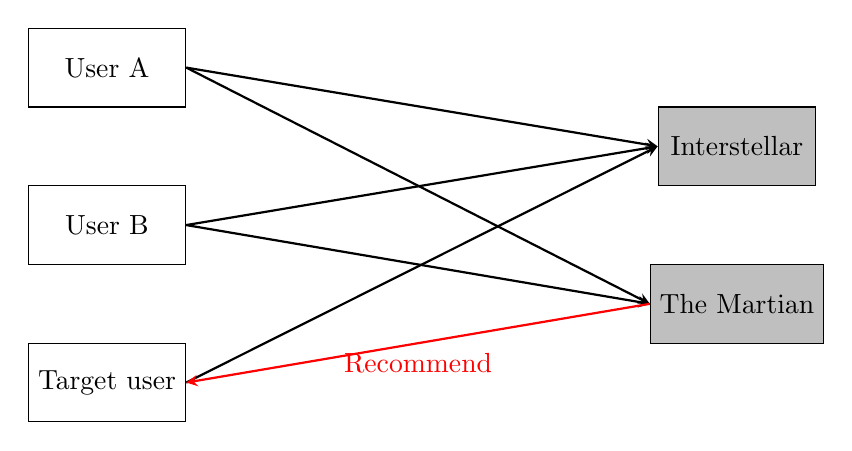
\begin{tikzpicture}[
    user/.style={draw, rectangle, fill=white, minimum width=2cm, minimum height=1cm},
    movie/.style={draw, rectangle, fill=gray!50, minimum width=2cm, minimum height=1cm},
    arrow/.style={->, thick, >=stealth},
    rec_arrow/.style={->, thick, >=stealth, red}
]
% Users (positioned on the left)
\node[user] (userA) at (-4,2) {User A};
\node[user] (userB) at (-4,0) {User B};
\node[user] (target) at (-4,-2) {Target user};

% Movies (positioned on the right)
\node[movie] (interstellar) at (4,1) {Interstellar};
\node[movie] (martian) at (4,-1) {The Martian};

% Watch arrows - Users to Movies
\draw[arrow] (userA.east) -- (interstellar.west);
\draw[arrow] (userB.east) -- (interstellar.west);
\draw[arrow] (target.east) -- (interstellar.west);
\draw[arrow] (userA.east) -- (martian.west);
\draw[arrow] (userB.east) -- (martian.west);

% Recommendation arrow - Movie to User (distinct styling)
\draw[rec_arrow] (martian.west) -- (target.east) node[midway, below] {\textcolor{red}{Recommend}};
\end{tikzpicture}
\caption{An illustration of item-based collaborative filtering.}
\label{fig:item-based-cf}
\end{figure}